\section{Variational Properties}

\begin{figure}
\begin{center}

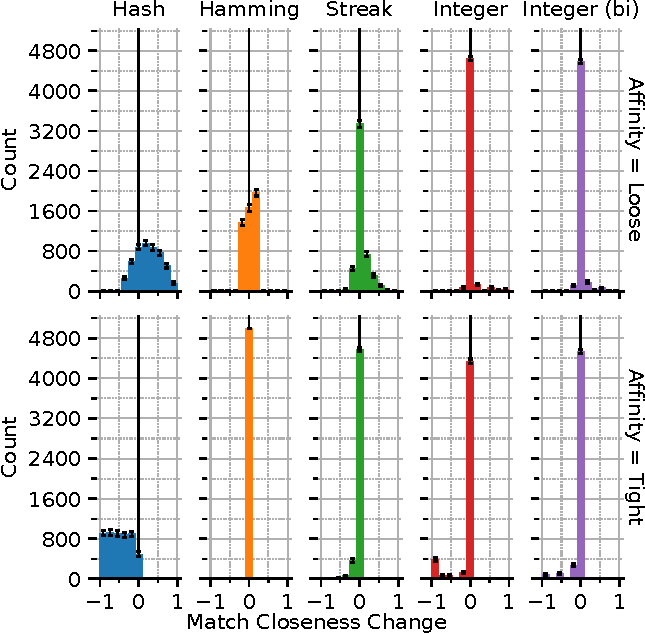
\includegraphics[width=\columnwidth]{img/mutational_step/bitweight=0dot5+seed=1+title=low-mutational-step+viz=hist+_data_hathash_hash=95a57768de56995a+_script_fullcat_hash=aa068ad24b386169+ext=}
\caption{
Distributions of mutation effects on match distance for loosely matched (pre-mutation match distance $> 0.5$) and tightly matched (pre-mutation match distance $< 0.01$) tag pairs.
Note that match closeness change (rather than mast distance change) is plotted so that better-matching mutational outcomes fall to the right and worse-matching mutational outcomes fall to the left.
Error bars are 95\% confidence intervals calculated using the Wilson score method with continuity correction \citep{newcombe1998two}.
Supplementary Figure \ref{fig:mutational_step_supp} shows the cumulative distribution of all sampled match distance changes for each metric.
}
\label{fig:mutational_step}

\end{center}
\end{figure}


We began by analyzing the distribution of single-bit mutations on match scores under the different metrics.
Figure \ref{fig:mutational_step} provides this analysis for two categories of tag pairs: loosely matched and tightly matched.
To generate the loosely matched distribution we unifomormly selected from tag pairs with a match distance > 0.5, measured their match distance, applied a one-bit mutation to the second tag, and then measured their match distance again.
To generate the tightly matched distribution we picked a target tag.
Then, we uniformly sampled a second tag with a match distance < 0.01.
We measured their match distance, applied a one-bit mutation to the second tag, and then measured their match distance again.
We sampled 5000 measurements for each affinity and each metric.

For both tight and loose affinities, although the integer metrics exhibited no perfectly neutral mutational outcomes most mutations cause very small change in the match score.
These are mutations to the least-significant bits of the bitstring.
A small fraction of mutations under these metrics, affecting the more-significant bits of the bitstring, have a stronger effect.
The integer metrics, along with the hash metric, exhibit the strongest one-step decoupling mutations under tight affinity.
The Spector integer metric, in particular, due to its asymmetrical wraparound-search inducing effect, exhibits more frequent strong decoupling mutations than the bidirectional integer metric.

The streak metric alone exhibits a portion of perfectly neutral outcomes under mutation.
The streak metric exhibits a greater fraction of mutational outcomes of non-trivial magnitude than the integer metrics with loose affinity.
Under tight affinity, the streak metric exhibits some one step strong-decoupling mutations but less intensely than the integer metrics.

The hamming metric exhibits more uniformity in the magnitudes of mutational effects than other metrics under both tight and loose affinities.
The hamming metric exhibits no perfectly neutral mutational outcomes.
(Without uniformification, all hamming metric mutations are of excactly the same magnitude with respect to match score).

The hash metric exhibits the greatest fraction of non-trivial mutational effects and exhibits some mutational intensities as extreme as the integer metrics.

\begin{figure*}
\begin{center}

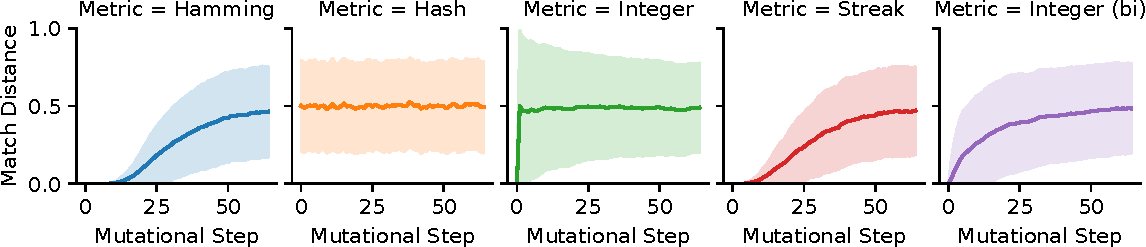
\includegraphics[width=\textwidth]{{{mutational_walk/bitweight=0.5+seed=1+title=mutational_walk_lineplot+_data_hathash_hash=ff15c8831d4f9288+_script_fullcat_hash=c872df869f05035a+ext=}}}
\caption{
TODO
}
\label{fig:mutational_walk_lineplot}

\end{center}
\end{figure*}

\begin{figure}
\begin{center}

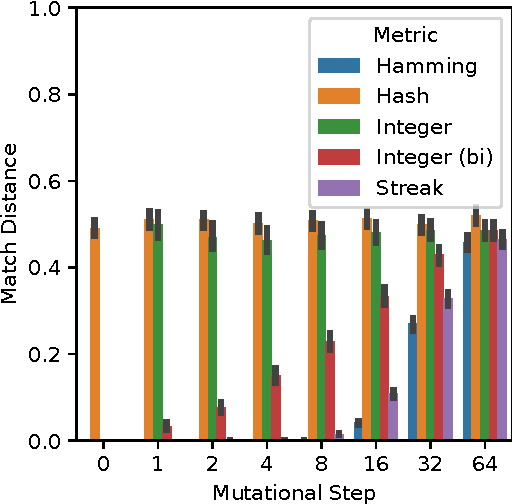
\includegraphics[width=\columnwidth]{{{mutational_walk/bitweight=0.5+seed=1+title=mutational_walk_barplot+_data_hathash_hash=8bf152d87daa9cb7+_script_fullcat_hash=982405ca713eba73+ext=}}}
\caption{
Snapshots of match distance at exponentially increasing steps from identical tags.
Error bars represent 95\% confidence intervals.
}
\label{fig:mutational_walk_barplot}

\end{center}
\end{figure}


Next, we performed mutational walks under each metric.
We began with two randomly chosen equivalent tags (mutation step zero) then applied randomly chosen one-step mutations (with the possibility of back mutation allowed) 65 times to the second tag.
We measured match distance between the two tags at each mutational step.
We performed 1000 independent mutational walks from different starting equivalent tags.

Figure \ref{fig:mutational_walk_lineplot} continuously depicts the distribution of match distances on mutational walks, with shaded areas indicating standard deviation, under different metrics.
Figure \ref{fig:mutational_walk_barplot} compares match distances at exponentially increasing steps.
Error bars indicate 95\% confidence intervals.

For the hash metric, where equivalent tags don't necessarily have low match distance, the mutational walk wanders around loose affinity.

The Spector Integer metric, where half of mutational steps wrap back around to 1.0 distance, immediately spikes up to an average match distance of 0.5.
The variance decreases with mutational steps as the distribution moves away from bias towards distances of 0 and 1.

The bidirectional integer metric experiences a greater immediate jump in variance and significantly greater mean match distance as rare mutations affecting significant bits take place (non-overlapping 95\% CI).

The
Intrestingly, contrary to as was claimed in \citep{downing2015intelligence}, the uniformified streak metric's match score under mutation actually grows significantly faster than the hamming metric's match score  (non-overlapping 95\% CI).

Because the are uniformified, the distributions all devolve to having an equivalent mean and variance.


